% !TeX root = report.tex
% !TeX spellcheck = en_GB

\section{Results}
The results of the experiments can be seen on Figures \ref{experiments:graph:1} and \ref{experiments:graph:2}. The $x$ axis shows the generation, and the $y$ axis shows the champion fitness achieved for that generation in the run.

\begin{figure}[ht]
	\begin{subfigure}{\textwidth}
		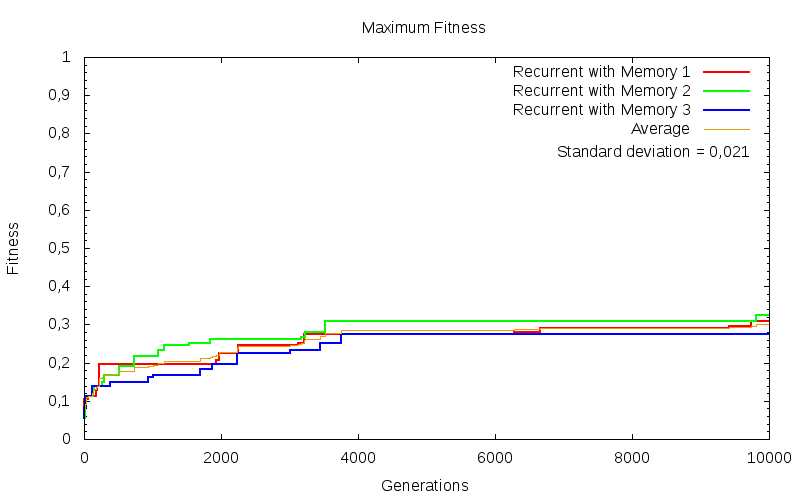
\includegraphics[width=\textwidth]{figures/recurrentmemory.png}
		\caption{}
	\end{subfigure}
	\begin{subfigure}{\textwidth}
		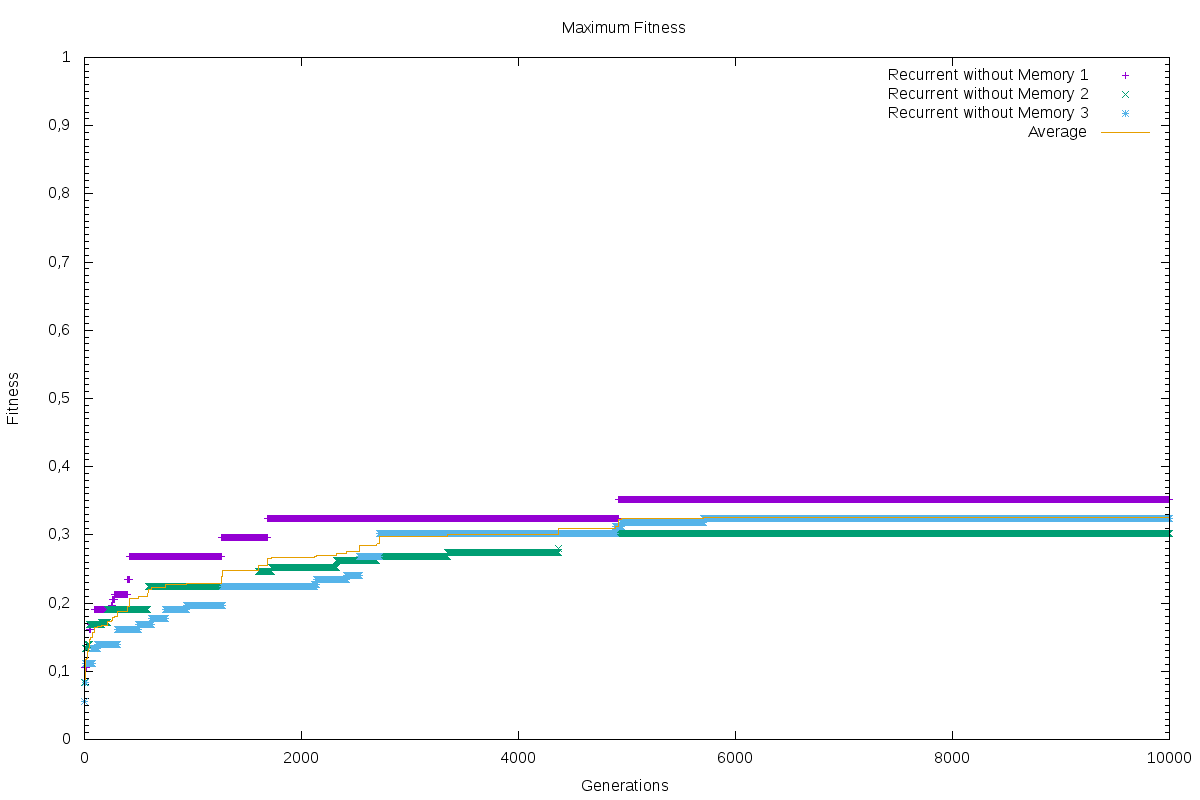
\includegraphics[width=\textwidth]{figures/recurrentnomemory.png}
		\caption{}
	\end{subfigure}
	\caption{Graph of the results when using recurrent networks. (a) is with enabled memory bank, (b) is without.}
	\label{experiments:graph:1}
\end{figure}

\begin{figure}[ht]
	\begin{subfigure}{\textwidth}
		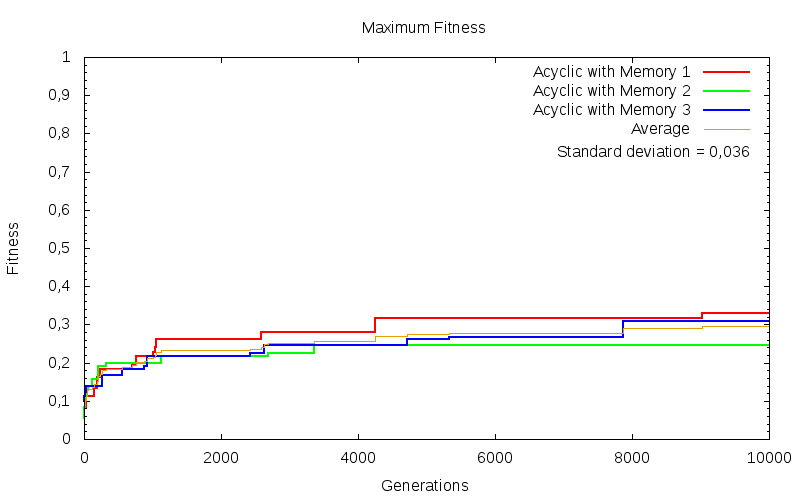
\includegraphics[width=\textwidth]{figures/acyclicmemory.png}
		\caption{}
	\end{subfigure}
	\begin{subfigure}{\textwidth}
		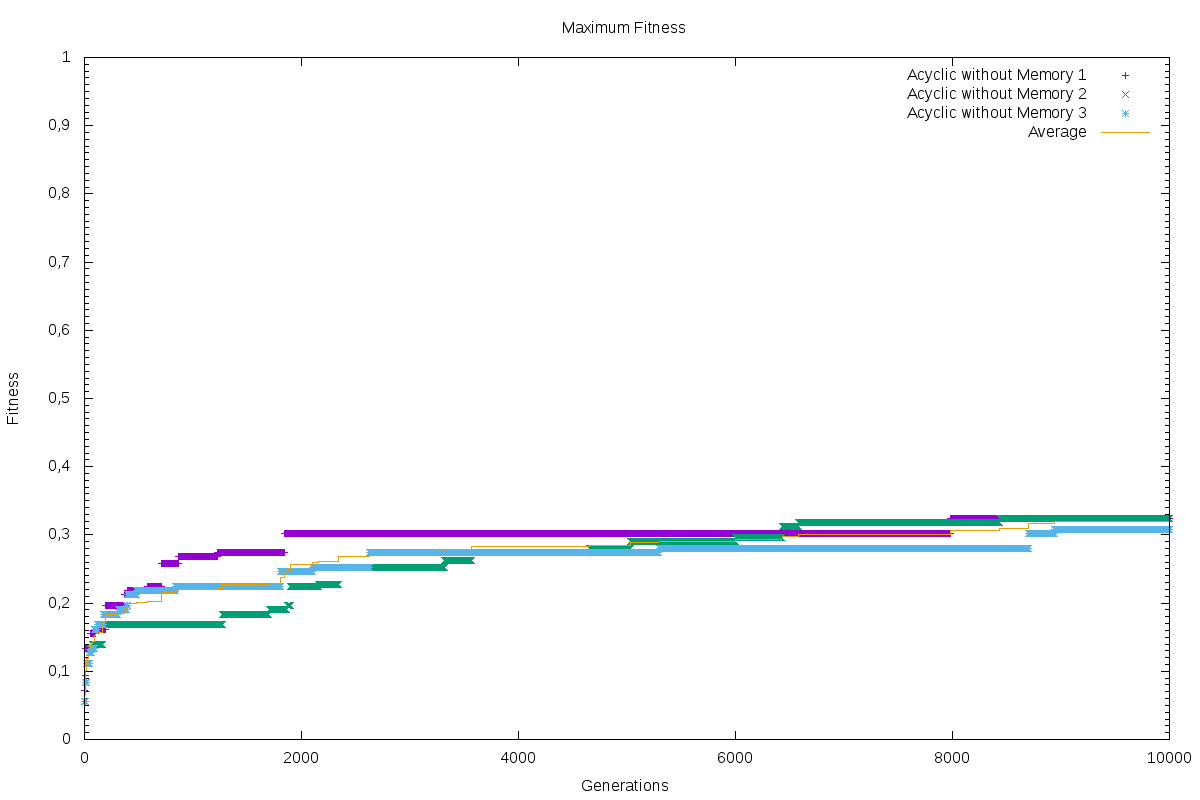
\includegraphics[width=\textwidth]{figures/acyclicnomemory.png}
		\caption{}
	\end{subfigure}
	\caption{Graph of the results when using acyclic networks. (a) is with enabled memory bank, (b) is without.}
	\label{experiments:graph:2}
\end{figure}

\begin{figure}[ht]
	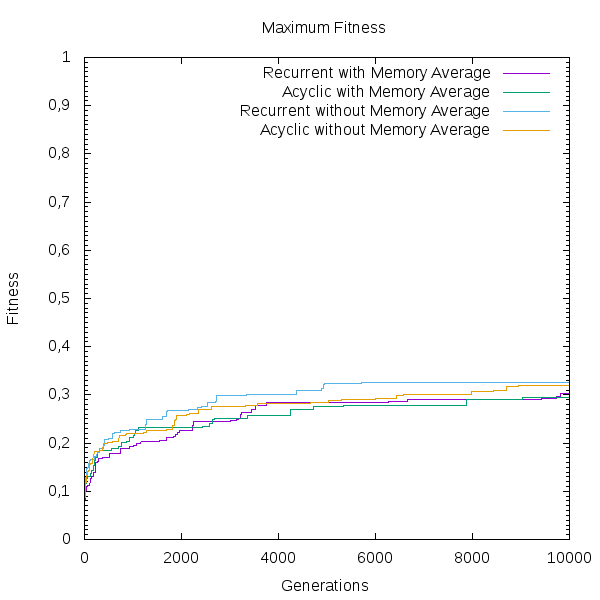
\includegraphics[width=\textwidth]{figures/averages.png}
	\caption{Averages over three runs of all configurations.}
	\label{experiments:graph:average}
\end{figure}

\newpar What is mostly hidden in the separate graphs, are show in \autoref{experiments:graph:average}. At least with the amount of generations we have allowed the network to operate within, the averages of the runs at generation 10.000 shows that both kinds of networks finds a better performing neural network when the Turing-functionality is turned off.

\newpar We will discuss possible reasons for this in the following sections.

\todo{Kan vi inddrage noget turing-memory halløj?}
\clearpage